\documentclass[fleqn,12pt]{article}
\usepackage[top=2cm, left=2cm,right=3cm,bottom=2cm]{geometry}
%\usepackage[fleqn]{amsmath}
\usepackage{amsmath}
\usepackage{url,enumerate}
\usepackage{color,hyperref,enumerate,multicol}
\usepackage{ifthen}
\newboolean{answers}
%\setboolean{answers}{true}  % set to true to include TODO statements
\setboolean{answers}{false}  % set to false to use input statements
\usepackage{amssymb}
\usepackage{tikz}
\newcommand{\<}{\ensuremath{\langle}}
\renewcommand{\>}{\ensuremath{\rangle}}
\newcommand{\Z}{\ensuremath{\mathbb{Z}}}
\newcommand{\ur}{\ensuremath{\underline{\mathrm{r}}}}
\newcommand{\uT}{\ensuremath{\underline{\mathrm{T}}}}
\newcommand{\uF}{\ensuremath{\underline{\mathrm{F}}}}
\newcommand{\uN}{\ensuremath{\underline{\mathrm{N}}}}
\newcommand{\ui}{\ensuremath{\underline{\mathrm{i}}}}
\newcommand{\uj}{\ensuremath{\underline{\mathrm{j}}}}
\newcommand{\ua}{\ensuremath{\underline{\mathrm{a}}}}
\newcommand{\ub}{\ensuremath{\underline{\mathrm{b}}}}
\newcommand{\un}{\ensuremath{\underline{\mathrm{n}}}}
\newcommand{\uv}{\ensuremath{\underline{\mathrm{v}}}}
\newcommand{\id}{\ensuremath{\operatorname{id}}}
\newcommand{\ba}{\ensuremath{\mathbf{a}}}
\newcommand{\bv}{\ensuremath{\mathbf{v}}}
\newcommand{\bb}{\ensuremath{\mathbf{b}}}
\newcommand{\bA}{\ensuremath{\mathbf{A}}}
\newcommand{\bB}{\ensuremath{\mathbf{B}}}
\newcommand{\bS}{\ensuremath{\mathbf{S}}}
\newcommand{\bT}{\ensuremath{\mathbf{T}}}
\newcommand{\bc}{\ensuremath{\mathbf{c}}}
\newcommand{\bi}{\ensuremath{\mathbf{i}}}
\newcommand{\bj}{\ensuremath{\mathbf{j}}}
\newcommand{\meet}{\ensuremath{\wedge}}
\newcommand{\join}{\ensuremath{\vee}}
\newcommand{\dotsize}{1pt}
\begin{document}
%\thispagestyle{empty}
\pagestyle{empty}
%\fontsize{11.5}{13.8}
% \fontsize{14}{17}
% \selectfont
\noindent {\bf MATH 301 - Section B}
\hfill {\bf Fall 2014}
\begin{center}
{\bf Midterm Exam 2}
\thispagestyle{empty}
%% covers sections 5.1--5.5 and 7.1--7.4
\end{center}
\vskip1cm
\noindent {\bf RULES}
\begin{enumerate}
\item All phones and other electronic devices must be silenced for the duration
  of the exam.
\item No books, notes, or calculators allowed.
%% \item Out of consideration for your classmates, do not make
%% disturbing noises during the exam. If you need a tissue, please ask for one.
%% \item Are you still reading the rules?  Did you read rule number 1?  If you
%%   haven't yet taken out your phone to turn it off, read rule
%%   number 1 a few more times.
\end{enumerate}
\vskip1cm
{\it Cheating will not be tolerated.}  If there are any indications that a
  student may have given or received unauthorized aid on this exam, the case 
  will be brought to the ISU Office of Academic Integrity.% \\
\\[4pt]
After finishing the exam, please sign the following statement
acknowledging that you understand and accept this policy:\\
\\
``On my honor as a student I,
\underline{\phantom{XXXXXXXXXXXXXXXX}}, have neither
given nor received unauthorized aid on this exam.''
\hbox{} \hskip .75cm {\small (print name clearly)}\\
\\
\begin{flushright} Signature: \underline{\phantom{XXXXXXXXXXXXXXXXXXXXXXXX}}
  Date: \underline{\phantom{XXXXXXXXXX}}
\end{flushright}

\begin{center}
  
{\bf Do not sign the pledge until after you have finished the exam.}
\end{center}

\newpage
\begin{enumerate}[{\bf 1.}]
\item Give precise definitions of the following:

  \begin{enumerate}
  %% \item {\bf algebra}
  %%   \vskip4cm
  \item {\bf $n$-ary operation} on a set $A$
    \vskip3cm

  \item {\bf $n$-ary relation} on a set $A$
    \vskip3cm

  %% \item {\bf relation}
  %%   \vskip4cm

  \item {\bf algebra} or {\bf algebraic structure}
    \vskip3cm

  \item {\bf relational structure}
    \vskip3cm

  %% \item {\bf relational structure} $\<A, R\>$
  %%   \vskip4cm

  \item {\bf group homomorphism}
    \vskip3cm

  %% \item {\bf algebra homomorphism} $\varphi: \<A, F^\bA\> \rightarrow \<B, F^\bB\>$
  %%   \vskip3cm

  %% \item {\bf group isomorphism}
  %%   \vskip2.5cm

  \item {\bf normal subgroup}
    
  \end{enumerate}

\newpage

\item
  \begin{enumerate}
  \item State \emph{Lagrange's Theorem} about the order of a group and its
    subgroups. (Be sure to state all assumptions that are needed in order for
    the theorem to hold.)  
\vskip7cm
    \item Recall that $G$ is the 
      \emph{internal direct product} of the subgroups $H$ and $K$ if 
      $H\cap K= \{e\}$ and $H$ and $K$ centralize each other (i.e., $hk = kh$ for
      all $h\in H$ and $k\in K$). 

      Suppose $G$ has order 28 and subgroups $H$ and $K$ of orders 4
      and 7 respectively which centralize each other.  Prove that
      $G$ is the internal direct product of $H$ and $K$.
  \end{enumerate}

%% \medskip
%% \noindent {\bf Solution:}  
%% Assume $hk = kh$ for all $h\in H$ and $k\in K$.
%% Suppose $x \in H\cap K$, then $x \in H$ implies $\<x\>$ is a subgroup of $H$ so,
%% by Lagrange's Theorem $|x|$ divides $|H| = 4$.
%% Similarly $x \in K$ implies $\<x\>$ is a subgroup of $K$ so,
%% by Lagrange's Theorem $|x|$ divides $|K| = 5$. Since $|x|$ divides both 4 and 5,
%% we must have $|x| = 1$, so $x = e$.  That is $H\cap K = \{e\}$. \qed
\newpage
\item {\bf Prove either (a) OR (b) OR (c).} If you prove more than one, circle the letter you
  want graded.

\begin{enumerate}
\item
Prove that if $G \cong H$ and $G$ is cyclic, then $H$ is cyclic.
%% \medskip
%% \noindent {\bf Solution:} Suppose $G = \<a\> \cong H$ and suppose 
%% $\varphi: G \rightarrow H$ is an isomorphism.  Then 
%% $H = \<\varphi(a)\>$.  To see this, fix $h\in H$.  We will show 
%% $h = (\varphi(a))^k$ for some $k\in \N$. Indeed, let $b = \varphi^{-1}(h)$.
%% Since $b\in G = \<a\>$, we must have $b = a^k$ for some $k\in \N$.
%% Also, $\varphi(a^k) = (\varphi(a))^k$, since $\varphi$ is a homomorphism. 
%% Therefore, $(\varphi(a))^k = \varphi(a^k) = \varphi(b) = \varphi(\varphi^{-1}(h)) = h$.
%% \qed
\item If a group $G$ has a subgroup $H$ of index 2, then $H$ is
normal in $G$. \\
Conclude that $A_n \triangleleft S_n$ for $n \geq 3$.
\item 
If a group $G$ has exactly one subgroup $H$ of order $k$, then
$H$ is normal in $G$. 

\end{enumerate}


%% \medskip
%% \noindent {\bf Solution:} 
%% We will solve this using\\[4pt]
%% \indent {\bf another standard way to prove a subgroup $H$ is normal in $G$:}
%% \medskip
%% \begin{quote}
%% \emph{Pick an arbitrary element $g\in G$ and show that $gHg^{-1} = H$.}
%% \end{quote}
%% \medskip
%% First, given a subgroup $H\leq G$, and an arbitrary element $g\in G$, it is not hard to
%% see that the \emph{conjugate of $H$ by $g$}, which is defined by
%% \[
%% gHg^{-1} := \{ghg^{-1} | h\in H\},
%% \]
%% is also a subgroup of $G$.  Moreover, the function $h \mapsto ghg^{-1}$ is a
%% bijection.\footnote{In fact, as we will see later, $x\mapsto gxg^{-1}$ 
%% is an automorphism.}  
%% Therefore, $|H| = |gHg^{-1}|$.  If $|H| =k$ and if $H$ is the only
%% subgroup of $G$ of order $k$, then, since $|gHg^{-1}| = k$, we must have 
%% $H = gHg^{-1}$.
%% Since $g$ was arbitrary, this proves that $H$ is normal in $G$.
%% \qed

\newpage

\item The {\bf center} of a group $G$ is
$Z(G) = \{ x \in G : xg = gx \text{ for all $g \in G$ }\}$.
%% We proved that $Z(G) \triangleleft G$, so the set $G / Z(G)$ of cosets forms a
%% group. Also, we proved that $G$ is abelian if $G/Z(G)$ is cyclic.

\begin{enumerate}
 \item
Show that the center of any group is a normal subgroup.
 \vskip7cm

\item
The dihedral group $D_4$ (symmetries of the square) can be
described as the permutation group with two generators 
$\rho = (1234)$ and $\mu = (13)$ satisfying $\rho^4= e = \mu^2$.
Therefore, the elements of $D_4$ are 
$\{e, \rho, \rho^2, \rho^3, \mu, \rho \mu, \rho^2 \mu, \rho^3 \mu\}$.

Calculate $Z(D_4)$, the center of $D_4$. [Hint: only one nonidentity
element of $D_4$ commutes with all other elements of $D_4$, and finding
this element should not require too much calculation.]
 
%%  \item
%% Calculate the center of $GL_2 ( {\mathbb R} )$.
 \vskip7cm

 
 \item
Is $D_4/Z(D_4)$ cyclic?  Explain. [Hint: Recall, we proved that 
$G$ is abelian if $G/Z(G)$ is cyclic.]
\end{enumerate}
\newpage
\item State the First Isomorphism Theorem and use it to prove that every group $G$
  is isomorphic to a subgroup of $\operatorname{Sym}(G)$. [Hint: show that a certain function
    $\lambda :G \rightarrow \operatorname{Sym}(G)$ is a homomorphism with trivial kernel.]

\newpage

\item Let $\bS = \<S, \cdot\>$ and $\bT = \<T, \circ\>$ be two semilattices.
  \begin{enumerate}
  \item Say what it means for a function $\varphi: S \rightarrow T$ to be a
    \emph{semilattice homomorphism} $\varphi: \bS \rightarrow \bT$.
\vskip3cm
\item Let $S = \{a, b, c, d\}$ and $T = \{0, 1, 2\}$, and suppose 
  $\bS = \<S, \cdot\>$ and
  $\bT= \<T, \circ\>$ have the Cayley tables given below

\medskip
\begin{center}
\begin{tabular}{r|rrrr}
  $\cdot$ & $a$ &$b$&$c$&$d $\\
\hline
  $a$ & $a$ &$a$&$a$&$a$\\
  $b$ & $a$ &$b$&$a$&$b$\\
  $c$ & $a$ &$a$&$c$&$c$\\
  $d$ & $a$ &$b$&$c$&$d$
\end{tabular}
\hskip2cm
\begin{tabular}{r|rrr}
  $\circ$ & $0$ &$1$&$2$\\
\hline
  $0$ & $0$ &$0$&$0$\\
  $1$ & $0$ &$1$&$1$\\
  $2$ & $0$ &$1$&$2$
\end{tabular}
\end{center}

\medskip
The Hasse diagrams of $\bS$ and $\bT$ are as follows:
\begin{center}
  
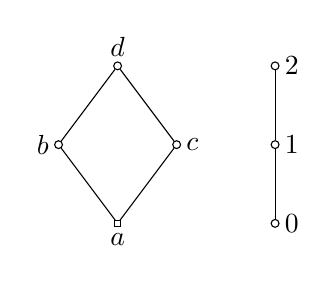
\begin{tikzpicture}[scale=0.5]
  \node (0) at (0,0) [draw, inner sep=1pt] {};
  \node (1) at (1.5,2)[draw,circle,inner sep=1pt] {}; 
  \node (2) at (-1.5,2) [draw,circle,inner sep=1pt] {};
  \node (3) at (0,4) [draw,circle,inner sep=1pt] {};
  \node (a) at (4,0) [draw,circle,inner sep=1pt] {};
  \node (b) at (4,2) [draw,circle,inner sep=1pt] {};
  \node (c) at (4,4) [draw,circle,inner sep=1pt] {};
  \draw (a) to (b) to (c);
  \draw (0) to (1) to (3) to (2) to (0);

  \draw (0) node [below] {$a$};
  \draw (2) node [left] {$b$};
  \draw (1) node [right] {$c$};
  \draw (3) node [above] {$d$};
  \draw (a) node [right] {$0$};
  \draw (b) node [right] {$1$};
  \draw (c) node [right] {$2$};
\end{tikzpicture}
\end{center}

Determine which of the functions $\varphi_i$ defined below is a homomorphism.
In case $\varphi_i$ is not a homomorphism, give an example of 
a violation of the definition in Part (a).

\medskip
\begin{center}
\begin{tabular}{c|c}
  $x$ & $\varphi_1(x)$ \\
\hline
  $a$ & $0$\\\hline
  $b$ & $1$\\\hline
  $c$ & $0$\\\hline
  $d$ & $1$
\end{tabular}
\hskip3cm
\begin{tabular}{c|c}
  $x$ & $\varphi_2(x)$ \\
\hline
  $a$ & $0$\\\hline
  $b$ & $1$\\\hline
  $c$ & $1$\\\hline
  $d$ & $2$
\end{tabular}
%% \hskip2cm
%% \begin{tabular}{c|c}
%%   $x$ & $\varphi_3(x)$ \\
%% \hline
%%   $a$ & $1$\\\hline
%%   $b$ & $1$\\\hline
%%   $c$ & $2$\\\hline
%%   $d$ & $2$
%% \end{tabular}
\end{center}
\end{enumerate}
  \end{enumerate}

\newpage
~

\newpage

\begin{center}
  EXTRA CREDIT
\end{center}
Below I have drawn the subgroup lattice diagrams for the groups $\Z_2$,
$\Z_7$, $\Z_{12}$, $\Z_{16}$, $\Z_{30}$, $S_3$, and  $D_4/Z(D_4)$ but I've
forgotten which diagram go with which group.  I was able to label the first
diagram correctly.  If you think you can help me label the others, go for
it. But don't guess. 

\medskip

{\it $+1$ point for each correct answer, $-1/4$ point for each incorrect answer.} 
%\begin{multicols}{2}

\bigskip

\begin{center}
% Z_2
\begin{tikzpicture}[scale=1.25]
  \node (bot) at (0,0) [draw,circle,inner sep=1pt] {};
  \node (top) at (0,2) [draw,circle,inner sep=1pt] {};
  \draw (bot) to (top);
  \node (G) at (0,-1) {$G = \Z_2$};
  \node (line) at (.1,-1.2) {\underline{\phantom{XXXXXXX}}};
\end{tikzpicture}
\hskip3cm
% Z_7
\begin{tikzpicture}[scale=1.25]
  \node (bot) at (0,0) [draw,circle,inner sep=1pt] {};
  \node (top) at (0,2) [draw,circle,inner sep=1pt] {};
  \draw (bot) to (top);
  \node (line) at (0,-1.2) {\underline{\phantom{XXXXXXX}}};
\end{tikzpicture}
% Z_16
\hskip3cm
\begin{tikzpicture}[scale=1.25]
  \node (bot) at (0,0) [draw,circle,inner sep=1pt] {};
  \node (1) at (0,1) [draw,circle,inner sep=1pt] {};
  \node (top) at (0,2) [draw,circle,inner sep=1pt] {};
  \draw (bot) to (1) to (top);
  \node (line) at (0,-1.2) {\underline{\phantom{XXXXXXX}}};
\end{tikzpicture}
\end{center}
\vskip1cm
\begin{center}
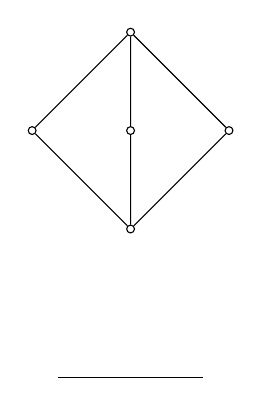
\begin{tikzpicture}[scale=1.25]
  \node (bot) at (0,0) [draw,circle,inner sep=1pt] {};
  \node (1) at (1,1) [draw,circle,inner sep=1pt] {};
  \node (2) at (-1,1) [draw,circle,inner sep=1pt] {};
  \node (3) at (0,1) [draw,circle,inner sep=1pt] {};
  \node (top) at (0,2) [draw,circle,inner sep=1pt] {};
  \draw (bot) to (1) to (top) to (2) to (bot) to (3) to (top);
  \node (line) at (0,-1.4) {\underline{\phantom{XXXXXXX}}};
\end{tikzpicture}
\hskip3cm
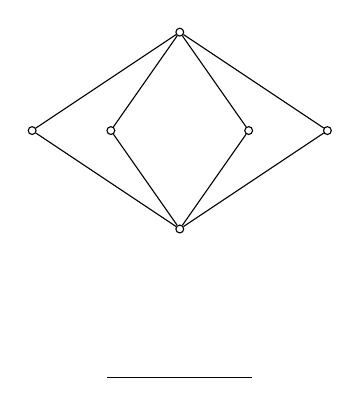
\begin{tikzpicture}[scale=1.25]
  \node (bot) at (0,0) [draw,circle,inner sep=1pt] {};
  \node (1) at (1.5,1) [draw,circle,inner sep=1pt] {};
  \node (2) at (-1.5,1) [draw,circle,inner sep=1pt] {};
  \node (3) at (.7,1) [draw,circle,inner sep=1pt] {};
  \node (4) at (-.7,1) [draw,circle,inner sep=1pt] {};
  \node (top) at (0,2) [draw,circle,inner sep=1pt] {};
  \draw (bot) to (1) to (top) to (2) to (bot) to (3) to (top) to (4) to (bot);
  \node (line) at (0,-1.4) {\underline{\phantom{XXXXXXX}}};
%  \node (G) at (0,-1.5) {$G =$};
\end{tikzpicture}
\end{center}
\vskip1cm
\begin{center}
\begin{tikzpicture}[scale=0.7]
  \node (1) at (0,0) [draw,circle,inner sep=1pt] {};
  \node (6) at (2,2)[draw,circle,inner sep=1pt] {}; 
  \node (4) at (-2,2) [draw,circle,inner sep=1pt] {};
  \node (2) at (0,4) [draw,circle,inner sep=1pt] {};
  \node (3) at (4,4) [draw,circle,inner sep=1pt] {};
  \node (G) at (2,6) [draw,circle,inner sep=1pt] {};
  \draw (1) to (6) to (2) to (4) to (1);
  \draw (6) to (3) to (G) to (2) to (4);
  \node (line) at (1,-1.4) {\underline{\phantom{XXXXXXX}}};
%  \node (G) at (0,-1.5) {$G =$};
\end{tikzpicture}
\hskip3cm
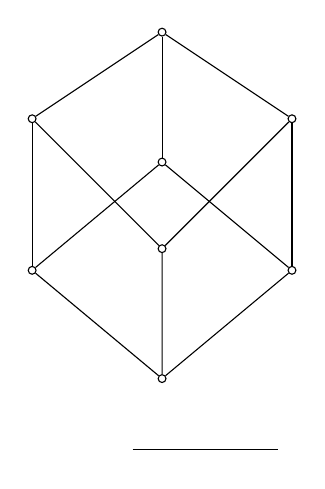
\begin{tikzpicture}[scale=0.55]
  \node (e) at (0,0)  [draw,circle,inner sep=1pt] {};
  \node (G) at (0,8) [draw,circle,inner sep=1pt] {};
  \node (2) at (-3,6) [draw,circle,inner sep=1pt] {};
  \node (3) at (0,5)  [draw,circle,inner sep=1pt] {};
  \node (5) at (3,6) [draw,circle,inner sep=1pt] {}; 
  \node (6) at (-3,2.5) [draw,circle,inner sep=1pt] {};
  \node (10) at (0,3)  [draw,circle,inner sep=1pt] {};
  \node (15) at (3,2.5)  [draw,circle,inner sep=1pt] {};
  \node (line) at (1,-1.4) {\underline{\phantom{XXXXXXX}}};
  \draw (e) to (15) to (3) to (6) to (e);
  \draw (e) to (10) to (5) to (G) to (2) to (10);
  \draw (6) to (2) (3) to (G) (15) to (5);
\end{tikzpicture}
\end{center}



\end{document}
\newpage
\vskip1cm
\item Give precise definitions of the following:

  \begin{enumerate}
  %% \item {\bf algebra}

  %%   \vskip4cm

  \item {\bf semigroup}

    \vskip4cm

  \item {\bf monoid}

    \vskip4cm

  \item {\bf group}

    \vskip4.5cm

  \item {\bf abelian group}

    \vskip3.5cm

  \item {\bf cyclic group}
    
  \end{enumerate}

\newpage

\item Let $G$ denote the symmetries of an equilateral triangle.

\begin{center}
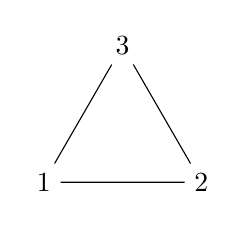
\begin{tikzpicture}[scale=0.5]
  \node (1) at (-2,0) {1};
  \node (2) at (2,0) {2};
  \node (3) at (0,3.4641) {3};
  \draw (1) to (2) to (3) to (1);
\end{tikzpicture}
\end{center}


  \begin{enumerate}
\item Write two or three sentences describing this group.   (If you wish to write down
the group elements, you may, but in the interest of time, consider doing this
after you have finished other parts of the test.)
\vskip7cm

\item What is the order of this group?
\vskip3cm
%%   %% \item What is the \emph{universe} of the group $G$?
%%   %% \item What is the set $X$ upon which the elements of $G$ act?
%%   \item Write down the Cayley table for this groupff. (This will be easier if you give
%%     short names to each of the group elements in part (a).)

%% \vskip5mm
%%     \begin{tabular}{c|c}
%% &\\
%% \phantom{XX}      & \phantom{XXXXXXXXXXXXXXXXXXXXXXXX}\\
%% \hline
%% &\\
%% &\\
%% &\\
%% &\\
%% &\\
%% &\\
%% &\\
%% &\\
%% &\\
%% &\\
%% &
%%     \end{tabular}
%% \vskip1cm 
\item Is this group cyclic? Is it abelian?  (Give a brief justification for your
  answers.)

  \end{enumerate}
\newpage

\item Suppose $H$ and $K$ are subgroups of a group $G$. Prove or disprove the following:
  \begin{enumerate}
  \item $H\cap K$ is a subgroup of $G$.
\vskip11cm
  \item $H\cup K$ is a subgroup of $G$.
  \end{enumerate}
\newpage

\item %Let $\mathbf{G} = \<G, \cdot, ^{-1}, e\>$ 
  Let $G$ be a group.  Prove the following:
  \begin{enumerate}
  %% \item If $G$ is an abelian group, then $(gh)^n = g^nh^n$ holds for all $g, h \in G$.
  %%   \vskip7cm
  \item $G$ is abelian if and only if $(gh)^2 = g^2h^2$ holds for all $g, h \in G$. 
    \vskip11cm
  \item If $G$ is cyclic, then $G$ is abelian.
\newpage
  \item Give a specific example of a group $G$ and elements $g, h \in G$ for which $(gh)^2 \neq g^2h^2$. 
    \vskip9cm
  \item Give a specific example of a group that is abelian but not cyclic.
  \end{enumerate}

\newpage
%% \begin{enumerate}
\item This problem has several parts.
First, state the following (without proof):
  \begin{enumerate}
  \item \emph{The Well Ordering Principle.} (about subsets of natural numbers)
    \vskip3cm

  \item \emph{The Division Algorithm.} (about integers $a$ and $b$ where $b>0$)
  \end{enumerate}
  \vskip3cm

Next prove that every subgroup of a cyclic group is cyclic by following the
steps below.
First, let $G = \<a\>$ be a cyclic group and fix an arbitrary subgroup $H\leq G$.
  \begin{enumerate}
  \item Suppose $H$ contains only the identity, $e$. Explain why $H$
    must be cyclic in this case.
    \vskip4cm
  \item Suppose instead that $H$ contains more than just the identity element. 
    Let $m$ be the smallest positive integer such that $a^m\in H$.  
    Why does such a number $m$ exists? (Cite a well known principle and say
    why this principle can be applied here.) 
    \vskip6cm
  \item Finally, prove the claim on the next page, which says that $a^m$
    generates $H$,  where $m$ is the number from part (b).
    %% ; that is, prove that if $x$ is an arbitrary element of $H$, then
    %%     $x$ is a power of $a^m$.
  \end{enumerate}

\newpage
{\bf Claim:} If $H\leq G = \<a\>$ and $m$ is the smallest positive integer such
that $a^m \in H$, then $H = \<a^m\>$.

\medskip

\noindent {\it Proof:}

\hfill

%% \newpage

%% \item
%%   Prove {\bf one} of the statements below. Only one answer will be graded.  (If
%%   you give more than one proof, then clearly label the one you want graded.)

%%   \begin{enumerate}
%% \item The order of an element of a cyclic group divides the order of the group.\\
%% (Do not simply cite Lagrange's Theorem.)

%% \item 
%% If $G = \<a\>$ is a cyclic group, then 
%% the subgroup $\<a^j, a^k\>$ generated by $a^j$ and $a^k$ is equal to
%% $\<a^d\>$, where $d = \gcd(j,k)$.
%% (Hint: Recall that there exist integers $r$ and $s$ such that $d = rm + sk$; you
%% may use this fact without proving it.)

%% \end{enumerate}
\newpage
\item
  Answer either (a) or (b). Only one answer will be graded.  (If
  you answer both, then clearly mark which should be graded.)
  \begin{enumerate}
\item 
Show that, for any cyclic group $G = \<a\>$, 
the subgroup $\<a^j, a^k\>$ generated by $a^j$ and $a^k$ is equal to
$\<a^d\>$, where $d = \gcd(j,k)$.
(Hint: Recall that there exist integers $r$ and $s$ such that $d = rm + sk$; you
may use this fact without proving it.)
\item
Show that for any group $G$, and any fixed element $g \in G$,
the map $\lambda_g : G \rightarrow G$ defined by
$\lambda_g(a) = g a$ is a permutation of $G$.
Then show that the order of the alternating group on $n$ letters is $|A_n| = n!/2$.
%% (Hint: first explain why the order of $S_n$ is $n!$, then prove that exactly half
%% of the elements of $S_n$ must be in $A_n$.)
\end{enumerate}

\newpage
\item
  \begin{enumerate}[(a)]
  \item Give a precise definition of \emph{equivalence relation}, then give an example.
    \vskip5cm
  \item Give a precise definition of \emph{partial order relation}, then give an example.
    \vskip5cm
    \item Let $f:X \rightarrow Y$ be a function and define the relation $\sim$
      on the set $X$ as follows:
    \[
    m \sim n \quad \text{ if and only if } \quad f(m) = f(n)
    \]
    What kind of relation is $\sim$?  (Justify your answer by checking the properties.)
  %% \item Give a precise definition of \emph{total order relation}, then give an example.
  %%   \vskip4cm
  %%   \item Of the three types of relations mentioned above, which of these is
  %%     typically associated with a partition of a set into disjoint subsets?
  %%   \vskip4cm
  \end{enumerate}

\newpage
\end{enumerate}
\begin{center}
  Extra Credit
\end{center}
\begin{enumerate}
\item[EC 1.] ($6$ points)
Below I have drawn the subgroup lattice diagrams for the groups $\Z_2$, $\Z_2 \times \Z_2$,
$\Z_7$, $\Z_{12}$, $\Z_{16}$, $\Z_{30}$, and $S_3$, but I've forgotten which diagram
go with which group.  I was able to label the first diagram
correctly.  If you think you can help me label the others, go for it. But
don't guess! 

\medskip

{\it $+1$ point for each correct answer, $-1/2$ point for each incorrect answer.} 
%\begin{multicols}{2}

\bigskip

\begin{center}
% Z_2
\begin{tikzpicture}[scale=1.25]
  \node (bot) at (0,0) [draw,circle,inner sep=1pt] {};
  \node (top) at (0,2) [draw,circle,inner sep=1pt] {};
  \draw (bot) to (top);
  \node (G) at (0,-1) {$G = \Z_2$};
  \node (line) at (.1,-1.2) {\underline{\phantom{XXXXXXX}}};
\end{tikzpicture}
\hskip3cm
% Z_7
\begin{tikzpicture}[scale=1.25]
  \node (bot) at (0,0) [draw,circle,inner sep=1pt] {};
  \node (top) at (0,2) [draw,circle,inner sep=1pt] {};
  \draw (bot) to (top);
  \node (line) at (0,-1.2) {\underline{\phantom{XXXXXXX}}};
\end{tikzpicture}
% Z_16
\hskip3cm
\begin{tikzpicture}[scale=1.25]
  \node (bot) at (0,0) [draw,circle,inner sep=1pt] {};
  \node (1) at (0,1) [draw,circle,inner sep=1pt] {};
  \node (top) at (0,2) [draw,circle,inner sep=1pt] {};
  \draw (bot) to (1) to (top);
  \node (line) at (0,-1.2) {\underline{\phantom{XXXXXXX}}};
\end{tikzpicture}
\end{center}
\vskip1cm
\begin{center}
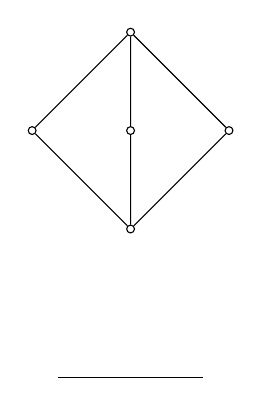
\begin{tikzpicture}[scale=1.25]
  \node (bot) at (0,0) [draw,circle,inner sep=1pt] {};
  \node (1) at (1,1) [draw,circle,inner sep=1pt] {};
  \node (2) at (-1,1) [draw,circle,inner sep=1pt] {};
  \node (3) at (0,1) [draw,circle,inner sep=1pt] {};
  \node (top) at (0,2) [draw,circle,inner sep=1pt] {};
  \draw (bot) to (1) to (top) to (2) to (bot) to (3) to (top);
  \node (line) at (0,-1.4) {\underline{\phantom{XXXXXXX}}};
\end{tikzpicture}
\hskip3cm
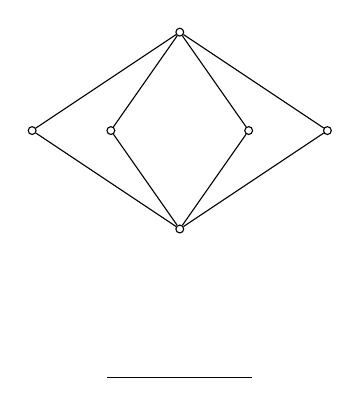
\begin{tikzpicture}[scale=1.25]
  \node (bot) at (0,0) [draw,circle,inner sep=1pt] {};
  \node (1) at (1.5,1) [draw,circle,inner sep=1pt] {};
  \node (2) at (-1.5,1) [draw,circle,inner sep=1pt] {};
  \node (3) at (.7,1) [draw,circle,inner sep=1pt] {};
  \node (4) at (-.7,1) [draw,circle,inner sep=1pt] {};
  \node (top) at (0,2) [draw,circle,inner sep=1pt] {};
  \draw (bot) to (1) to (top) to (2) to (bot) to (3) to (top) to (4) to (bot);
  \node (line) at (0,-1.4) {\underline{\phantom{XXXXXXX}}};
%  \node (G) at (0,-1.5) {$G =$};
\end{tikzpicture}
\end{center}
\vskip1cm
\begin{center}
\begin{tikzpicture}[scale=0.7]
  \node (1) at (0,0) [draw,circle,inner sep=1pt] {};
  \node (6) at (2,2)[draw,circle,inner sep=1pt] {}; 
  \node (4) at (-2,2) [draw,circle,inner sep=1pt] {};
  \node (2) at (0,4) [draw,circle,inner sep=1pt] {};
  \node (3) at (4,4) [draw,circle,inner sep=1pt] {};
  \node (G) at (2,6) [draw,circle,inner sep=1pt] {};
  \draw (1) to (6) to (2) to (4) to (1);
  \draw (6) to (3) to (G) to (2) to (4);
  \node (line) at (1,-1.4) {\underline{\phantom{XXXXXXX}}};
%  \node (G) at (0,-1.5) {$G =$};
\end{tikzpicture}
\hskip3cm
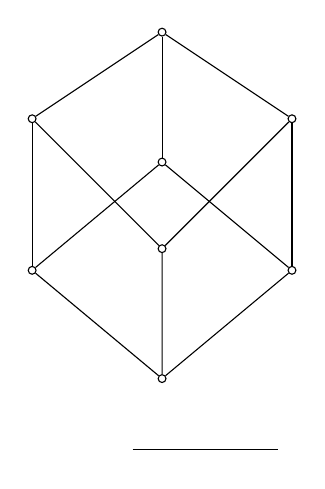
\begin{tikzpicture}[scale=0.55]
  \node (e) at (0,0)  [draw,circle,inner sep=1pt] {};
  \node (G) at (0,8) [draw,circle,inner sep=1pt] {};
  \node (2) at (-3,6) [draw,circle,inner sep=1pt] {};
  \node (3) at (0,5)  [draw,circle,inner sep=1pt] {};
  \node (5) at (3,6) [draw,circle,inner sep=1pt] {}; 
  \node (6) at (-3,2.5) [draw,circle,inner sep=1pt] {};
  \node (10) at (0,3)  [draw,circle,inner sep=1pt] {};
  \node (15) at (3,2.5)  [draw,circle,inner sep=1pt] {};
  \node (line) at (1,-1.4) {\underline{\phantom{XXXXXXX}}};
  \draw (e) to (15) to (3) to (6) to (e);
  \draw (e) to (10) to (5) to (G) to (2) to (10);
  \draw (6) to (2) (3) to (G) (15) to (5);
\end{tikzpicture}
\end{center}

\item[EC 2.] (1/2 point) Which group appears in William DeMeo's GitHub gravatar?\\
{\small (William DeMeo the mathematician, not the actor.)}
\end{enumerate}

\end{document}


\begin{tikzpicture}[scale=0.75]
  \node (1) at (0,0) {$\langle e \rangle$}; 
  \node (6) at (2,2) {$\langle g^6 \rangle$}; 
  \node (4) at (-2,2) {$\langle g^4 \rangle$}; 
  \node (2) at (0,4) {$\langle g^2 \rangle$}; 
  \node (3) at (4,4) {$\langle g^3 \rangle$}; 
  \node (G) at (2,6) {$\langle g \rangle$}; 
  \draw (1) to (6) to (2) to (4) to (1);
  \draw (6) to (3) to (G) to (2) to (4);
  \node (line) at (1,-1.4) {\underline{\phantom{XXXXXXX}}};
%  \node (G) at (0,-1.5) {$G =$};
\end{tikzpicture}

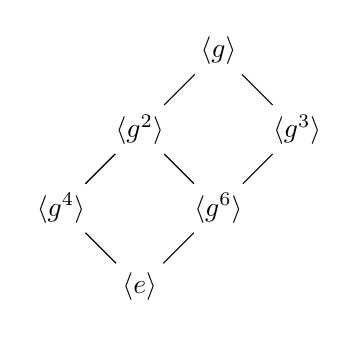
\begin{tikzpicture}[scale=0.5]
  \node (1) at (0,0) {$\langle e \rangle$}; 
  \node (6) at (2,2) {$\langle g^6 \rangle$}; 
  \node (4) at (-2,2) {$\langle g^4 \rangle$}; 
  \node (2) at (0,4) {$\langle g^2 \rangle$}; 
  \node (3) at (4,4) {$\langle g^3 \rangle$}; 
  \node (G) at (2,6) {$\langle g \rangle$}; 
  \draw (1) to (6) to (2) to (4) to (1);
  \draw (6) to (3) to (G) to (2) to (4);
\end{tikzpicture}

\begin{center}
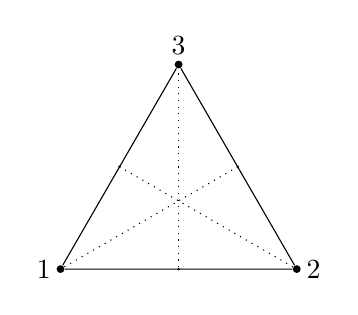
\begin{tikzpicture}[scale=0.75]
  \node (0) at (0,0) [fill,circle,inner sep=.2pt] {};
  \node (1) at (-2,0) [fill,circle,inner sep=1pt] {};
  \node (2) at (2,0) [fill,circle,inner sep=1pt] {};
  \node (3) at (0,3.4641) [fill,circle,inner sep=1pt] {};
  \node (4) at (1, 1.732) [fill,circle,inner sep=.2pt] {};
  \node (5) at (-1, 1.732) [fill,circle,inner sep=.2pt] {};
  \draw (1) node [left] {$1$};
  \draw (2) node [right] {$2$};
  \draw (3) node [above] {$3$};
  \draw (1) to (2) to (3) to (1);
  \draw[dotted] (0) to (3);
  \draw[dotted] (1) to (4);
  \draw[dotted] (2) to (5);
\end{tikzpicture}
\end{center}


\item
  \begin{enumerate}[(a)]
    \item Let $f:X \rightarrow Y$ be a function and define the relation $\sim$
      on the set $X$ as follows:
    \[
    m \sim n \quad \text{ if and only if } \quad f(m) = f(n)
    \]
    What kind of relation is $\sim$?  (Justify your answer by checking the properties.)
    \vskip10cm
  \item Does $\sim$ induce a partition of $X$ into disjoint sets?  If so,
    describe the sets in the partition.  If not, say why not.
  \end{enumerate}

\newpage


